%%
%% Terminology.tex
%% Login : <hoang-trong@hoang-trong-laptop>
%% Started on  Wed Jun 10 19:23:16 2009 Hoang-Trong Minh Tuan
%% $Id$
%% 
%% Copyright (C) 2009 Hoang-Trong Minh Tuan
%% This program is free software; you can redistribute it and/or modify
%% it under the terms of the GNU General Public License as published by
%% the Free Software Foundation; either version 2 of the License, or
%% (at your option) any later version.
%% 
%% This program is distributed in the hope that it will be useful,
%% but WITHOUT ANY WARRANTY; without even the implied warranty of
%% MERCHANTABILITY or FITNESS FOR A PARTICULAR PURPOSE.  See the
%% GNU General Public License for more details.
%% 
%% You should have received a copy of the GNU General Public License
%% along with this program; if not, write to the Free Software
%% Foundation, Inc., 59 Temple Place, Suite 330, Boston, MA 02111-1307 USA
%%

\chapter{Terminology}
\label{chap:terminology}


\begin{table}[!hbt]
  \begin{center}
    \caption{Terminology}
    \begin{tabular}{cp{9cm}}
      \hline
      notation& description \\
      \hline\hline
      $V_m$ & membrane potential ($V_m=V_i-V_o$) \\
      & [Voltage], mV \\
      $V_r$ ($V_{rest})$ & the membrane resting  potential \\ 
      & ...(computed using  Goldman equation)\\
      $v$ & membrane potential, $v=V_m-E_r$ \\
      & ... (\textcolor{red}{only used in early works}) \\
      & ...displacement from the resting   potential $E_r$ \\
      $E_i$ ($E_{rev}$) & reversible potential ($E_{\ce{Na}},
      E_{\ce{K}}$)  \\
      & ...(\textcolor{red}{computed using Nernst equation}) \\
      $v_i$  & potential across ion channel ($v_{\ce{Na}}, v_{\ce{K}}$), $v_i=V_i-V_r$
      \\
      &... displacement from the membrane resting potential $V_r$\\
      & ... (\textcolor{red}{only used in early works}) \\
      $V_L$ ($V_{leak}$) & leakage voltage [mV] \\
      $g_L$ & leakage conductivity (assumed to be constant) \\
            & ...unit:Siemens per area [mS.cm$^{-2}$] \\
      $g_i$ & electrical conductivity ($g_{\ce{Na}}, g_{\ce{K}}$) \\
      & ...or specific conductance (high value = good conductor) \\
      $\overline{g_i}$ & maximum conductance to be scaled \\
      & ...by gating channels \\
    \end{tabular}
  \end{center}
  \label{tab:terminology_1}
\end{table}
\begin{equation}
I_\ion = g_\ion \left( V_m - E_\ion \right)
\end{equation}
with $g_\ion$ can be modeled using Hodgkin-Huxley-based formulas, e.g. 
$g_\ion = \overline{g_\ion}.h^m.j^n$ (with $h,j$ are two gating variables, and
$m,n$ are Hill's coefficients).

\def\lsbracket{{\text{[]}}}
 \begin{table}[!hbt]
  \begin{center}
    \caption{Terminology}
    \begin{tabular}{cp{9cm}}
      \hline
      notation& description \\
      \hline\hline
      $k^+ (k_{on}),$ & rate constant (on/off) in a chemical reaction
      \\
      $k^- (k_{off})$      & 
       \ce{A + B <=>[k^+\ce{[A]^\eta}][k^-]AB}  \\
      & unit of $k^+$ is $1/(\mu$M$^\eta$.s), $k^-$ is $1/s$; with
      $\eta$ is Hill coefficient \\
      & ...In state-transition of a Markov-chain model, the ``on''
      rate transition can be constant or ligand-dependence, 
      ... e.g. [$\Ca$], [IP3], [ATP]...)\\
      $K_{d}$ ($K_{d,A}$) & ($\frac{k^-}{k^+}$) dissociation constant;
      unit ($\mu$M$^\eta$)\\
      & ... tells affinity of B to A\\
      & ... small value = high-affinity \\
      $R_c$, $R_i$, $r_i$ & (intracellular) cytoplasmic specific resistivity
      (Ohm.length)\\
          & (resistance across a unit length of cylinder)
      \\
      & unit: Ohm.length, e.g. Ohm.mm \\
      $r_e$ &  resistance across unit length of cylinder \\
      &  (extracellular) \\
      $R_m$ & membrane resistivity in the form of specific membrane resistance,
      i.e.      resistance across a surface area\\
      & ...of membrane (Ohm.area) (Ohm.cm$^2$)\\
      $\Csc$ & the specific membrane capacitance ($\mu$F/cm$^2$) \\
      & ... i.e.  capacitance per unit area \\
      $\Cm$ & the total membrane capacitance ($\mu$F) \\
      & $\Cm=\Csc.A_m$ \\
      % $R_m$ & the resistance per unit area ($\Omega$/cm$^2$) \\
      %$R_m$ & the membrane resistivity ($\Omega$.cm$^2$) \\
      $R=\frac{R_m}{A_m}$ & with $A_m$ is membrane surface area \\
      $c_m$ & the capacitance per unit length ($\mu$F/cm) \\
      $\lambda$ & characteristic length \\
    \end{tabular}
  \end{center}
  \label{tab:terminology_11}
\end{table}

\begin{table}[!hbt]
  \begin{center}
    \caption{Terminology}
    \begin{tabular}{cr} 
      \hline
      notation & description \\ 
      \hline\hline
      $F$ & Faraday constant ($=N_A.q_e$) \\
      & ...number of Coulombs per mole of electrons \\
      & ...$=96,485.3399$ ([C.mol$^{-1}$] or [mJ/(mV.mol)]) \\
      $N_A$ & Avogadro number \\
      & ...$=6.022\times 10^{23}$ mol$^-1$\\
      $q_e$ or $e$ & unit charge (charge of a proton) \\
      & ...$=1.602 \times 10^{-19}$ C. \\
      $z$ & valence (unitless) \\
      & ...e.g.:$z_\Ca=2$ \\
      $R$ & universal gas constant \\
      & ...$8.314472(15)$ (J.K$^{-1}$.mol$^{-1}$) \\
      $T$ & absolute temperature ($^0$C + 273.15) \\
      & ...unit: Kelvin or K \\
      $k_B$ & Boltzmann constant \\
      & ...$k_B=1.381\times 10^{-23}$J.K$^{-1}$ \\
      $Q=\frac{[B]}{[A]}$ & reaction quotient \\
      & in the reaction: $\ce{A <=> B}$ \\
      $f_0$ (or $f$)& the fraction of open channels \\
      $f_\infty$ & steady state fraction of open channels\\
      & (i.e. at equilibrium)\\
      $\dot{X}$ & first-order time derivative $\frac{dX}{dt}$ \\
      $\ddot{X}$ & second-order time derivative $\frac{d^2X}{dt^2}$\\
      $Y'$ & partial derivative ($dY/dx$) \\
      & ...Y is a multivariate function \\
      $Y''$ & $d^2Y/dx^2$ \\
      % $[X]$  & the concentration of the substance X \\
    \end{tabular}
  \end{center}
  \label{tab:Term_3}
\end{table}

\section{ODE}
\label{sec:ode}

We can use different ODE solvers:
\begin{enumerate}
  \item MatLab: ode45; ode23 functions
  
  \item 
\end{enumerate}

Here are some important forms of function with its differential equation
\begin{equation}
  \label{eq:84}
  \begin{split}
    F(x) &.......... F'(x) \\
    ct^d &.......... cdt^{d-1} \\
    \exp(ct) &........ c\times\exp(ct) \\
    \exp(ct)X(t)&........ \exp(ct) (\dot{X}(t) + cX(t))\\
    \sin(ct)&........ c\cos(ct)\\
    \cos(ct)&......... -c\sin(ct) \\    
  \end{split}
\end{equation}

\section{Concentration}
\label{sec:concentration}

\begin{table}[hbt]
\begin{center}
\caption{Notation for concentrations}
\begin{tabular}{cr} 
\hline
notation & description \\ 
\hline\hline
$[X]$ & concentration of substance X \\
$[X]_i$ or $[X]_{myo}$ & intracellular (myoplasmic) concentration \\
$[X]_{ds},[X]_{ss}$ & concentration of X in the dyadic (diadic) subspace \\
$[X]_{nsr}$ & concentration of X in the network SR \\
$[X]_{jsr}$ & concentration of X in the junctional SR \\
$[X]_{o}$ &  concentration of X in the extracellular space \\
$\frac{d[X]}{dt}$ & rate of change of X \\
& (+) sign if [X] increases \\
& (-) sign if [X] decreases \\
\end{tabular}
\end{center}
\label{tab:Concentration}
\end{table}

Concentration of ions 
\begin{itemize}
\item in squid giant axon and Mammalian neuron:
  Fig.~\ref{fig:squid_axon-ion_con}. 
\item in cardiac cells: Fig.~\ref{fig:ion_con_cardiac}
\end{itemize}
\begin{figure}[htb]
  \centerline{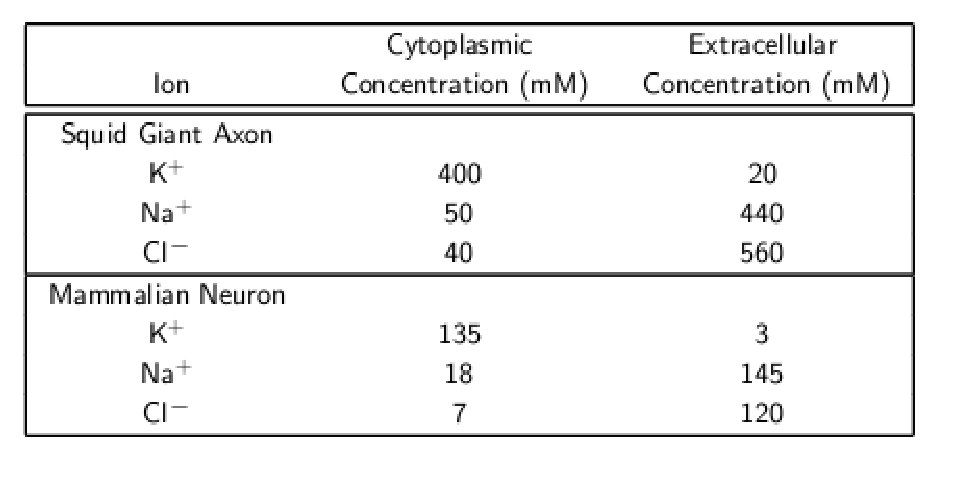
\includegraphics[height=4cm]{./images/ion_concentration.eps}}
  \caption{Ion concentration in squid giant axon and mammalian
    neuron}\label{fig:squid_axon-ion_con}
\end{figure}

\begin{figure}[htb]
  \centerline{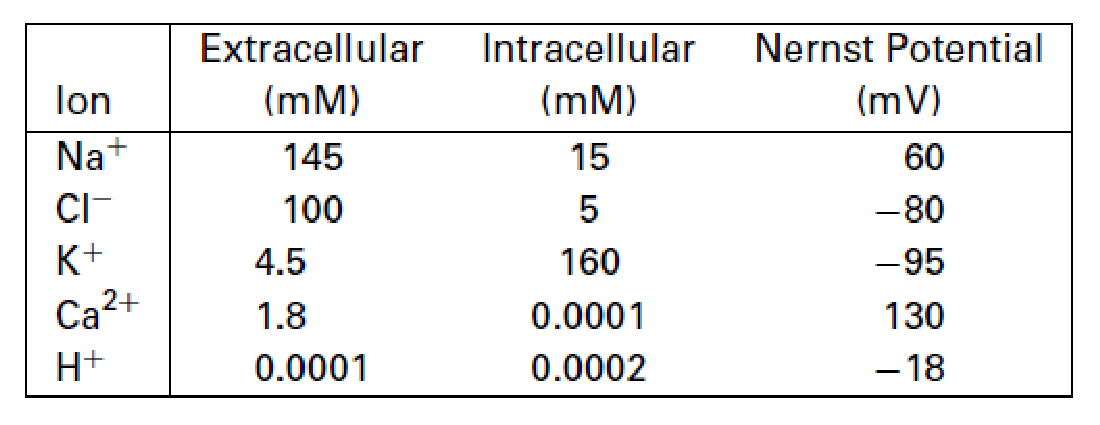
\includegraphics[height=3cm]{./images/ion_concentration_cardiac.eps}}
  \caption{Ion concentration in most cardiac
    cells}\label{fig:ion_con_cardiac}
\end{figure}


\section{Diffusion}
\label{sec:diffusion-2}

In 1D, an effective transport equation with an effective diffusion coefficient D
[$\mum^2$/s] and effective degradation rate k [1/s]:
\begin{equation}
\label{eq:reaction-diffusion-simple}
\frac{\partial c}{\partial t} = D \frac{\partial^2 c}{\partial x^2} - kc
\end{equation}
with the concentration $c$ (molecules/$\mum^3$) is a function of space and time, 
$c(x,t)$. For simplicity, we only write $c$. It is a partial differential
equation because it contains derivatives with respect to space and time
(Sect.\ref{sec:classification-pde}).
\begin{itemize}
  \item the first term is called the diffusion term
  \item the second term is called the reaction term. Here it represent the
  linear degradation (loss) (if $k>0$) and the production (if $k<0$) of the
  molecules of interest.

Sometimes, instead of the degradation rate $k$, the half-life of molecules
$\tau$ [s] is used. This is the time after which the concentration has been
reduced by half:
\begin{equation}
\frac{1}{2}c_i = c_i e^{-k\tau}
\end{equation}
or $k = ln(2)/\tau$.
In exponential gradients, the concentration decays by the same
 percentage at each position. 


   \item Non-linear degradation: the degradation rate $k$ is a function $k(c)$
   of the concentration 
\begin{equation}
\frac{\partial c}{\partial c} = -k(c).c
\end{equation}
with the special case: self-enhanced degradation
\begin{equation}
k(c) = k^* c^{n-1}; \;\;\; n>1
\end{equation}

\begin{equation}
\label{eq:reaction-diffusion-nonlinear}
\frac{\partial c}{\partial t} = D \frac{\partial^2 c}{\partial x^2} - k(c)
\times c
\end{equation}
 In the special case, the steady-state solution is 
 \begin{equation}
 c(x) = \frac{A}{(x+x_b)^m}
 \end{equation}
 As the concentration is proportional to $1/x^m$,
 the type of gradient is called {\it power-law gradient}.
Here, power-law gradients decay fast close to the source and more slowly at a
distance, i.e., their decay length-scale $\lambda_s$ is position-dependent and
reflects the local steepness of the gradient.
\begin{equation}
\begin{split}
\lambda_s = \frac{x+x_b}{m} \\
c_o = \frac{A}{x_b^m}
\end{split}
\end{equation}

  \item Linear degradation with directional bias:
  
  So far, no experimental evidence for spreading with directional bias has been
found, although it has been theoretically considered, although it has been
theoretically considered, e.g. morphogen molecules move by random walk, but
endogenous conditions make transport directional. This can be described by
regular diffusion plus a drift term, describing molecules moving with velocity
$v$ in a certain direction. 

A mechanism based on diffusion with drift and linear degradation leads to
exponential steady-state gradients, and the decay length is stretched or
compressed depending on the drift direction.

  
  \item directional {\bf active transport}, rather passive transport as
  described above.
  
  Example: vesicle movement on microtubule
  
  Active transport may be nondirectional, but it cannot be described by the
  diffusion equation, because it invokes forces.
  
  In passive transport (Fickian diffusion), the mean square displacement of
  freely diffusing molecules is linearly related to time.
  
  However, for actively transported molecules, this relationship is nonlinear.
  This is also true, for example, for molecules that are caged in polymer
  networks and thus do not diffuse freely.
  Such phenomena can be described by {\bf anomalous diffusion models}, which
  lead to the formation of exponential gradients.
   Continuous time random walk (CTRW) theory is used to model   \citep{hornung2005}
    
\end{itemize}
To understand how to solve the problem, read Sect.\ref{sec:morphogene}.

The diffusion coefficient of Bicoid has also been measured by FRAP (D = 0.3
$\mum^2$/s) (Gregor et al. 2007), whereas its degradation rate $k$ is unknown.

 The diffusion of calcium is in the range of 250-300$\mu$m$^2$/s in the
cytosol, and 100-150$\mu$m$^2$/s in the network SR. 
The diffusion values of other molecules are shown in Fig.~\ref{fig:diffusion_values}.

\begin{figure}[hbt]
 \centerline{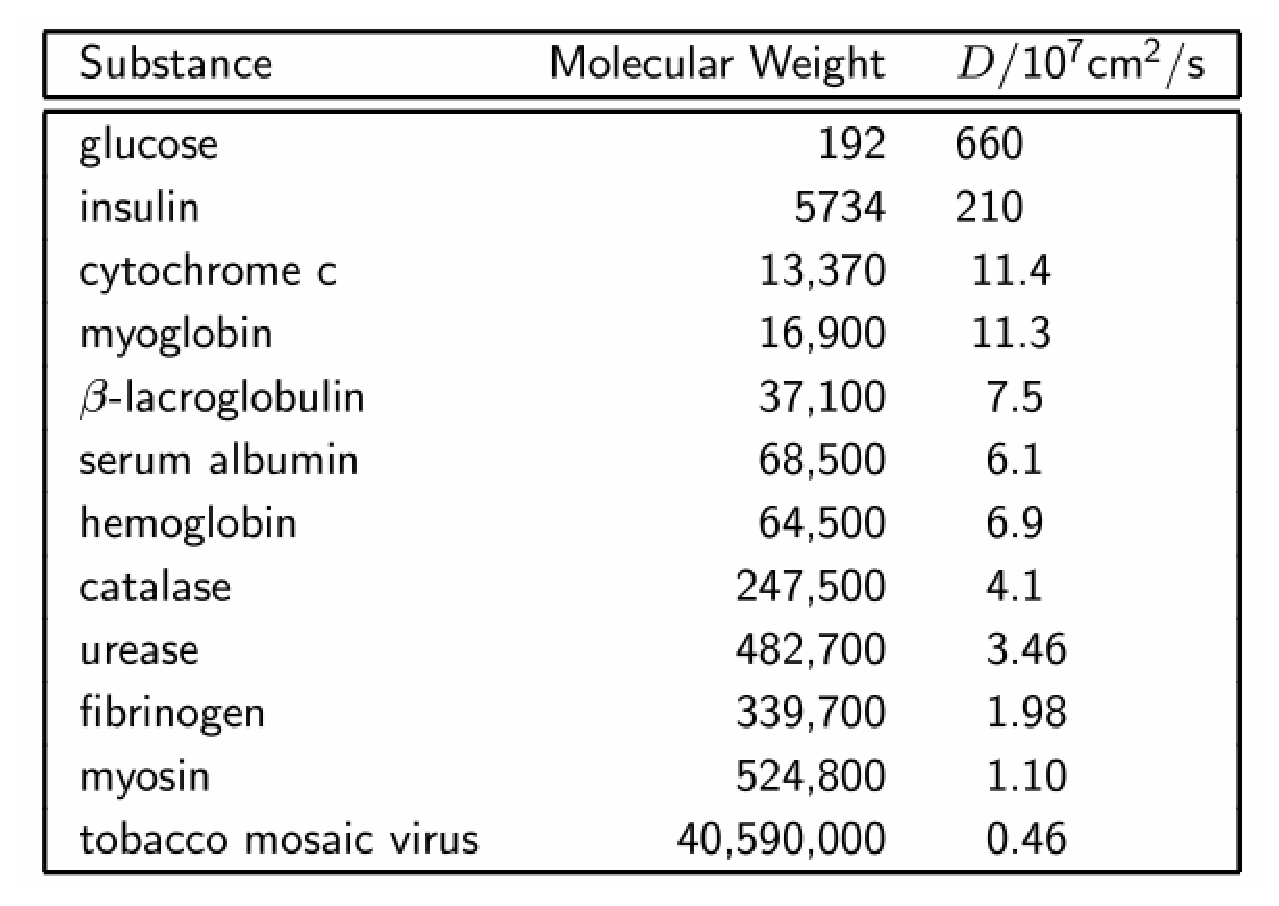
\includegraphics[height=5cm, angle=0]{./images/diffusion_values.eps}}
\caption{Molecular weight and diffusion coefficients of some
  biochemical substances}
\label{fig:diffusion_values}
\end{figure}

For isotropic (or spherical symmetric), the diffusion part is written as
\citep{crank1975}
\begin{equation}
\nabla \cdot (D_c\nabla C) = D_C \left( \frac{\partial^2 C}{\partial r^2} +
\frac{2}{r}\frac{\partial C}{\partial r} \right)
\end{equation} 
and for anisotropic diffusion, the formula is
\begin{equation}
\nabla \cdot (D_c\nabla C) = D_{Cx}\frac{\partial^2 C}{\partial x^2} +
D_{Cy}\frac{\partial^2 C}{\partial y^2} + 
D_{Cz}\frac{\partial^2 C}{\partial z^2} 
\end{equation}


\section{Electronic concepts}
\label{sec:basic-concepts}

The values for typical parameters are given in
Fig.~\ref{fig:cable_param}. 

\begin{figure}[hbt]
  \centerline{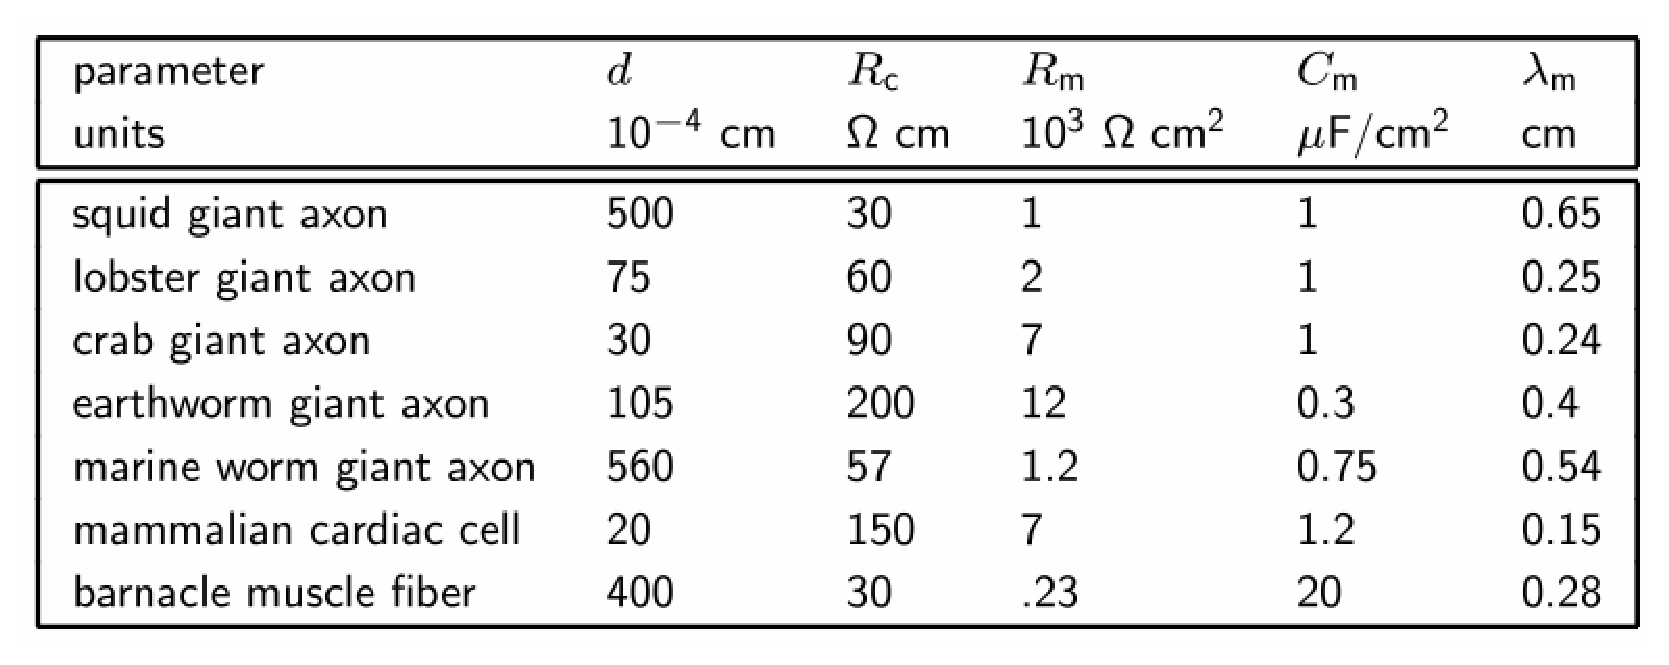
\includegraphics[height=5cm,
    angle=0]{./images/cable_parameters.eps}}
  \caption{Typical cable parameter values for a variety of excitable
    cell types (Keener an Sneyd (1998))}
  \label{fig:cable_param}
\end{figure}

\subsection{Electric time constant}
\label{sec:time-constant}

Consider a circuit of RC in parallel (Sect.\ref{sec:core-conductor-membrane}).
The time constant $\tau$ is
\begin{equation}
\tau = r_m c_m
\end{equation}

It is the time require to charge 63.2\% (or $e$-fold or $\sim 2/3$) of the
capacitor or to discharge it to 36.8\% (or $1/e$-fold) of its initial voltage is
known as the {\bf time constant} of the circuit.
\begin{eqnarray}
  \label{eq:490}
  \tau = \text{RC}
\end{eqnarray}
with R in unit Ohm, C in unit farad (F or
Coulomb/Voltage)\footnote{\url{http://www.tpub.com/neets/book2/3d.htm}}


\subsection{Membrane time constant}
\label{sec:membr-time-const-1}

Similarly, the concept of ``time constant'' is also important to
neurology. It tells how fast the neuron response to the synaptic input
or applied current (current injection), i.e. neuron's ``response
time''. In other words, it tells, when there is a synaptic input, how
long would it take for the neuron's membrane potential $V_m(t)$ to
increase/decrease $e$ times~\citep{koch1966htc}
(Sect.\ref{sec:membrane-time-constant}).

It is defined as
  \begin{equation}
    \label{eq:684}
    \tau = \Rm \Csc = \frac{\Csc}{g_\sc}
  \end{equation}
  with $g_\sc=\sum_i g_i$ (mS/cm$^2$) is the total conductance per unit
  area of membrane, $\Csc$ is specific membrane capacitance
  ($\mu$F/cm$^2$). The conductance is proportional to the number of open ion
  channels, and the capacitance is the function of the properties of the
  lipid bilayer. 
  
The time constant is used to describe how fast/slow the  rise and fall of the
membrane potential in response to the stimulus (i.e. injected current)
  \begin{equation}
    \label{eq:718}
    \begin{split}
      V_m &= V_{max}.(1-e^{-t/\tau})  \; \; \text{ rise} \\
      V_m &= V_{max}.e^{-t/\tau}  \; \; \text{ fall} \\
    \end{split}
  \end{equation}
  The meaning of this is that:
  \textcolor{red}{{\it the larger the time constant, the slower the rise or fall of the
      potential}}.

\section{Standard units}
\label{sec:standard-units}

To avoid the variation between cells, all quantities are determined
based on a unit of membrane area, except the voltage. The information
is given in Table~\ref{tab:terminology_2}.


\begin{table}[hbt]
  \begin{center}
    \caption{Standard units}
    \begin{tabular}{lr}
      \hline
      voltage (potential) & mV \\
      characteristic time constant ($\mathcal{T}$) & millisecond (ms) \\
      membrane time constant ($\tau_m$) & Farad.S or Farad.Ohm$^{-1}$ \\
      exponential time constant  ($\tau$) & sec \\
      + relaxation (decay/growth) time constant & \\
      currents ($I_i$) & $\mu$A.cm$^{-2}$ \\
      capacitances (C) & $\mu$F.cm$^{-2}$ \\
      conductances ($g_i$) & mho.cm$^{-2}$, m mho.cm$^{-2}$, n mho.cm$^{-2}$ \\
      cellular dimension & micrometer (micron) $\mu$m \\
      & $10^{-8}$cm$^2$ =  micron square\\
      the order of conductance $g$  & 1 to 150 pS \\
      whole-cell conductance of nanosiemens & mS.cm$^{-2}$ \\
      maximum possible conductance $\overline{g}$ & (mho/cm$^2$,mmho/cm$^2$,
      nmho/cm$^2$) \\
      concentration [X] & mM (milimolar, or milimole per litre)\\
      fraction of open channel ($f,f_\infty$) & unitless\\
      cell volume $V_{cell}$ & pL = $10^3\mu$m$^3$\\
      myoplasm volume $V_{myo}$ & \\
      network SR volume $V_{nsr}$ & \\
      
    \end{tabular}
  \end{center}
  \label{tab:terminology_2}
\end{table}

% In electrostatic, the work required to move a quantity of charge Q
% from point O to P is
% \begin{equation}
%   \label{eq:1219}
%   W_e = Q (\Phi_P-\Phi_O)
% \end{equation}
% with $V_m = \Phi_{out}-\Phi_{in}$ is the potential (mV), charge Q [C]
% (coulombs) and $W_e$ is work (J/mol). 
% In electrophysiology, the quantity of ions is often expressed in {\it
%   moles}. If one mole of ions is transferred, from point O to P, the
% work required is
% \begin{equation}
%   \label{eq:1220}
%   W_e = z_{ion}F(\Phi_P-\Phi_O)
% \end{equation}
% with $z_{ion}$ is the valence of the ion (e.g. $z_\ca=2$) [unitless],
% F is Faraday constant [C/mol]. Faraday constant convert the quantity
% of moles to the quantity of charges for a univalent ions; that's why
% we need to multiply the valence for non-univalent ions. 
% 
% When a force exerts on a unit charge, an electric field is
% defined. The work required to move a unit positive charge against the
% electric field $\overline{E}$ is
% \begin{equation}
%   \label{eq:1221}
%   dW = -\overrightarrow{E}\cdot\overrightarrow{ds}
% \end{equation}
% with $\overrightarrow{ds}$ is the vector displacement. Replacing
% $Q=1$ in eq.~\eqref{eq:1219}, then we have
% \begin{equation}
%   \label{eq:1222}
%   \Phi_P-\Phi_O =  -\overrightarrow{E} \cdot \overrightarrow{ds}
% \end{equation}
% Using Taylor series expansion
% \begin{equation}
%   \label{eq:1223}
%   \Phi_P= \Phi_O \frac{d\Phi}{ds} + ...
% \end{equation}
% If we neglect the higher order term, and keep the first term only.


% The {\bf current density} $\overrightarrow{J}$ and electric field
% $\overrightarrow{E}$ are related by
% \begin{equation}
%   \label{eq:1224}
%   \overrightarrow{J} = \sigma \overrightarrow{E} = -\sigma \nabla \Phi
% \end{equation}
% with $\sigma$ is the conductivity of the medium. If we're interested
% in the ions, the flux $j$ of these ions are subject to the electric field
% force, and is dependent upon the electric resistance, which in turns
% is a function of ionic mobility $u$ of the ionic species. 
% \begin{equation}
%   \label{eq:1225}
%   \overrightarrow{j_e} = u \frac{z}{|z|}c\nabla \Phi
% \end{equation}
% with $c$ is the ionic concentration [mol/cm$^3$], z = valence
% [unitless], u = ionic mobility [cm$^2$/(V.sec)], and
% $\overrightarrow{j_e}$ = ionic flux (due to electric field)
% [mol/(cm$^2$.sec)]. 
% 
% If, the ionic concentration is not uniform between adjacent
% compartments, there is a passive redistribution of ionic
% concentration, called {\bf diffusion}
% \begin{equation}
%   \label{eq:1226}
%   \overrightarrow{j_D} = -D\nabla c
% \end{equation}
% with D = diffusion constant [cm$^2$/sec], c = ionic concentration
% [mol/cm$^3$], $\overrightarrow{j_D}$ [mol/(cm$^2$.sec)].
% 
% \begin{framed}
%   A connection between ionic mobility $u$ and diffusion constant $D$
%   is
%   \begin{equation}
%     \label{eq:1227}
%     D = \frac{u.R.T}{|z|F}
%   \end{equation}
% with T = absolute temperature [K], R = Faraday constant [J/(mol.K)]
% \end{framed}
% 
% The {\bf Nernst-Planck equation} describes the flux of an ion under
% the affect of diffusion and electric field.
% \begin{equation}
%   \label{eq:1228}
%   \begin{split}
%     \overrightarrow{j} = \overrightarrow{j_D} + \overrightarrow{j_e} =
%     -D (\nabla c + \frac{c.z.F}{R.T}\Delta \Phi) 
%  \end{split}
% \end{equation}
% with $\overrightarrow{j}$ = ionic flux [mol/(cm$^2$.sec)]. We can
% easily convert the ionic flux to the electric current density $J$ by
% multiplying the ionic flux by $zF$ (i.e. the number of charges carried
% by each mole)
% \begin{equation}
%   \label{eq:1242}
%   \begin{split}
%     J = -DzF (\nabla c + \frac{c.z.F}{R.T}\Delta \Phi) \\
%     = - \left(u.R.T.\frac{z}{|z|}\nabla c + u.c.|z|F\nabla\Phi\right)
%   \end{split}
% \end{equation}
% with $J$ = electric current density [C/(sec.cm$^2$)] = [A/cm$^2$].
% 
% \begin{framed}
%   {\bf Nernst equation}: At equilibrium, there must be no current, or
%   \begin{equation}
%     \label{eq:1229}
%     \overrightarrow{j} = 0 =     -D (\nabla c +
%     \frac{c.z.F}{R.T}\Delta \Phi)  
%   \end{equation}
% or
% \begin{equation}
%   \label{eq:1230}
%   \nabla c = -\frac{z.F}{R.T}\Delta \Phi 
% \end{equation}
% or
% \begin{equation}
%   \label{eq:1231}
%   \frac{dc}{c} = -\frac{z.F}{R.T} .d\Phi 
% \end{equation}
% If we integrate from the intracellular space (i) to the outer
% extracellular space (o)
% \begin{equation}
%   \label{eq:1232}
%   \int^o_i  \frac{dc}{c} = \ln c|^o_i = -\frac{z.F}{R.T} \int^o_i d\Phi 
% \end{equation}
% or 
% \begin{equation}
%   \label{eq:1233}
%   \ln \frac{c_o}{c_i} = -\frac{z.F}{R.T} (\Phi_o-\Phi_i)
% \end{equation}
% \end{framed}

% The {\bf Goldman-Hodgkin-Katz equation} assumes that the membrane is
% planar, uniform and infinite in the lateral extent. Also, if $x$-axis
% is chosen normal to the membrane surface with the origin at the
% interface of the membrane with the extracellular region, $x=h$ is the
% thickness of the membrane (Sect.\ref{sec:membrane-thickness}), the variation of
% the potential field $\Phi$ is the function of $x$ only. 
% \begin{equation}
%   \label{eq:1234}
%   \frac{d\Phi}{dx} = \frac{\Phi_i-\Phi_o}{h}=\frac{V_m}{h}
% \end{equation}
% then, using eq.~\eqref{eq:1228}
% \begin{equation}
%   \label{eq:1235}
%   \overrightarrow{j} = -D(\frac{dc}{dx}+\frac{c.z.F}{R.T}\frac{d\Phi}{dx})
% \end{equation}
% or
% \begin{equation}
%   \label{eq:1236}
%   \frac{dc}{dx}=  -\frac{\overrightarrow{j}}{D}- \frac{V_m.z.F}{h.R.T}c
% \end{equation}
% or
% \begin{equation}
%   \label{eq:1237}
%   \frac{dc}{ -\frac{\overrightarrow{j}}{D}- \frac{V_m.z.F}{h.R.T}c} = dx
% \end{equation}
% If we assume a constant field approximation, i.e. $\overrightarrow{j}
% = \text{constant} = j$, so only $c$ is the function of $x$, we
% integrate both side from $x=0$ to $x=h$, then
% \begin{equation}
%   \label{eq:1238}
%   -\frac{hRT}{V_mzF}\ln\left(\frac{\frac{j}{D}+\frac{V_mzF}{hRT}c^{(h)}}{\frac{j}{D}+\frac{V_mzF}{hRT}c^{(0)}}\right) = h
% \end{equation}
% or
% \begin{equation}
%   \label{eq:1239}
%   j = -\frac{DV_mzF}{RTh} \frac{c^{(h)}-c^{(0)}\exp(-V_m\frac{zF}{RT})}{1-\exp(-V_m\frac{zF}{RT})}
% \end{equation}
% However, the measurable concentration are those in the intracellular
% and extracellular (bulk) space, and the formula use the concentration
% from just outside or just inside the membrane. So, if we assume they
% are scaled by a {\it partition coefficient $\beta$}, then
% \begin{equation}
%   \label{eq:1240}
%   \begin{split}
%     c^{(h)} = \beta_o c_o \\
%     c^{(i)} = \beta_i c_i \\
%   \end{split}
% \end{equation}
% with $c_i,c_o$ are measurable ionic concentration inside and outside,
% respectively. Finally, the {\bf Goldman-Hodgkin-Katz equation} is
% \begin{equation}
%   \label{eq:1241}
%   j = -\frac{DV_mzF}{RTh} \frac{\beta_ic_i-\beta_o c_o\exp(-V_m\frac{zF}{RT})}{1-\exp(-V_m\frac{zF}{RT})}
% \end{equation}
% Typically, we assume the partition coefficients are the same,
% i.e. $\beta_o =\beta_i = \beta$. 
% \begin{equation}
%   \label{eq:1245}
%   j = -\frac{\beta DV_mzF}{RTh} \frac{c_i- c_o\exp(-V_m\frac{zF}{RT})}{1-\exp(-V_m\frac{zF}{RT})}
% \end{equation}
% The electric current density, against, is computed by multiplying the
% flux with $zF$.
% 
% 
% The {\bf permeability} of an ion is defined as $P$ [cm/sec]
% \begin{equation}
%   \label{eq:1243}
%   P = \frac{D.\beta}{h}
% \end{equation}
% then the electric current density is
% \begin{equation}
%   \label{eq:1244}
%   J =  -\frac{P.V_mz^2F^2}{RT} \frac{\beta_ic_i-\beta_o c_o\exp(-V_m\frac{zF}{RT})}{1-\exp(-V_m\frac{zF}{RT})}
% \end{equation}
% Using this equation, if we consider a channel is permeated to more
% than one ion, say $\Ca$ channel is permeated by $\Ca, \Na$ and $\K$
% ions with 3 different permeability $P_\ca, P_\na, P_\k$ then at equilibrium
% \begin{equation}
%   \label{eq:1246}
%   J = J_\ca + J_\na + J_\k = 0
% \end{equation}
% or 
% \begin{equation}
%   \label{eq:1247}
%   \begin{split}
%     P_\k\left[c_{i,\k} - c_{o,\k}\exp (-\frac{E_mF}{RT}\right] &+
%     P_\na\left[c_{i,\na} -
%       c_{o,\na}\exp (-\frac{E_mF}{RT}\right] + \\
%     &P_\ca\left[c_{i,\ca} - c_{o,\ca}\exp (-\frac{E_mF}{RT})\right] = 0
%   \end{split}
% \end{equation}
% or
% \begin{equation}
%   \label{eq:1248}
%   P_\k c_{i,\k} +   P_\na c_{i,\na} +   P_\ca c_{i,\ca}  =
%   \exp(-\frac{E_mF}{RT}) \left(  P_\k c_{o,\k} +   P_\na c_{o,\na} +   P_\ca c_{o,\ca} \right)
% \end{equation}
% and the membrane potential at which the (net) membrane current is zero
% is called the {\bf reversal potential} $E_m$ which is defined via the
% so-called {\bf Goldman-Hodgkin-Katz} (GHK) equation as follows
% \begin{equation}
%   \label{eq:1249}
%   E_m = -\frac{RT}{F} \ln \frac{P_\k c_{i,\k} +   P_\na c_{i,\na} +   P_\ca c_{i,\ca}}{P_\k c_{o,\k} +   P_\na c_{o,\na} +   P_\ca c_{o,\ca}}
% \end{equation}
% 
% 
% 
% When performing any of the calculation between those quantities, it's
% important to know their units.  Standard units are: milivolts,
% miliseconds, nanofarads, nanoamperes, microsiemens (mS)
% \begin{verbatim}
% nF .mV/mS = nA = uS . mV
% \end{verbatim}
% 
% 
% However, in physiology, a better convention for some units is to
% define them {\it per unit of surface area}. This will avoid the
% geometrical difference between cells. The surface area of a neuron
% might be $3\times 10^4 \mu$m$^2$, or $3\times 10^{-2}$cm$^2$.  So, the
% new units are nanofarads per centimeters, nanoamperes per square
% centimeters, milisiemens per square centimeters.
% \begin{verbatim}
% (uF/cm^2) . mV/mS = uA/cm^2 = (mS/cm^2) . mV
% \end{verbatim}
% The quantities that are unaffected are milivolts, miliseconds. 
% 
% So, we use $\Csc$ (nF/cm$^2$) and $R_m$ ($\Omega$.cm$^2$).
% 



\section{Physical \& Chemical terms}
\label{sec:physical--chemical}

An ion's {\bf valence} is the number of charges, plus or minus, that
it carries. So, \ce{Ca^2+} is a {\it divalent}, while \ce{K+} is a
{\it univalent}.

If the permeability of \ce{K+} is considered one, the permeability of
other ions across the membrane is represented by the equation
\begin{eqnarray}
  \label{eq:539_copy}
  P_{\ce{K+}}:P_{\ce{Na+}}:P_{\ce{Cl-}} = 1:0.05:0.45
\end{eqnarray}

\section{Statistical tests}
\label{sec:statistical-tests}

The test for significant was two-tailed ANOVA among multiple
groups. For pairwise comparison, they used Student's t test. Differences
were considered significant when p-value $< 0.05$. 

\section{Tools for electrophysiology}

Data were analyzed with Igor Pro (Version 4, Wavemetrics, Lake
Oswego, OR), Clampfit 8 (Axon Instruments, Union City, CA) or
Mini Analysis (Synaptosoft, Decatur, GA).

For samples $>$10, central tendency was estimated by computing
a mean (mean $\pm$ SE); for smaller samples, medians were computed. 

Differences between samples were analyzed with a Student's t-test (large
samples) or a paired Wilcoxon signed-rank test (small samples).

\subsection{Tools for spike shape parameters extraction}

Spike shape parameters were measured using the Mini Analysis routines.
Specifically, spike threshold was determined by locating the membrane voltage at
which the second derivative of the spike waveform exceeded three times its SD in
a period before the spike onset.

Spike amplitude was defined as
the difference between the peak and the baseline of action potential.
Spike width was measured at half the spike amplitude. The afterhyperpolalization
was defined as the difference between the spike baseline
and the minimum membrane voltage after the action potential
peak.


%%% Local Variables: 
%%% mode: latex
%%% TeX-master: "mainfile"
%%% End: 
